\section{Experiments}
\label{sec:experiments}

\subsection{Tasks, graphs, and statistical units}
\label{sec:setup}

\paragraph{A task with known source information.}
Each source independently receives a balanced binary class $c_a,c_b$.
For class $c$, its 16-dimensional feature is $P_cz$, where
$z\sim\mathcal N(0,I_8)$ and $P_c$ is an orthonormal basis for a fixed
eight-dimensional subspace. The two class bases are drawn separately for
each seed block and are not required to be mutually orthogonal. All
non-source features are zero. The label is $y=c_a\oplus c_b$.
After two rounds of Eq.~\eqref{eq:operator}, a
$32\!\to\!64\!\to\!1$ ReLU MLP reads the two concatenated sink features.
No nonlinear message-passing layer precedes this readout.

The archived protocol fixes ten seed blocks
$\{11,17,23,31,41,53,67,79,97,103\}$. Each defines the subspace bases,
an on-the-fly training stream, and a separate 2,048-example evaluation
stream. Readouts are trained for 120 epochs of 32 batches of 128 samples
using Adam with learning rate 0.006. The ordinary graph conditions share
the data streams within each seed block. They are retrained separately,
so the evaluation measures finite-readout performance after an intervention.
The readout is constructed before an in-function seed reset; pairing the
data streams does not establish identical initial parameter values.

\paragraph{Controlled and biological wiring.}
The controlled graph contains 96 nodes and 337 directed edges. Its two
sources connect only to a designated relay; the relay is the only
incoming route to the two sinks. Background edges are generated outside
these restricted destinations. Removing the four motif edges therefore
eliminates source-to-sink communication under two-step propagation.

The real graphs are extracted from the public MaleCNS v1.0
connectome~\cite{malecns2026}. Visual annotation predicates define a
candidate neuron set; the 768 highest-total-degree neurons are selected,
then each target retains its highest-weight incoming partners. The
propagator uses the resulting binary support. Table~\ref{tab:graphs}
keeps the extraction settings separate. A relay is selected
deterministically from ascending node indices with two source neighbors,
two sink neighbors, five distinct nodes, and no direct source--sink edges
in the dense extracted graph. For the two $k=8$ extractions, the first
candidate with at least three common-relay triples is selected. This
criterion ensures distinct doses rather than selecting by accuracy.

\begin{table}[t]
\centering
\caption{\textbf{Real-wiring cohorts.} Each contains 768 nodes.
$k$ is the maximum number of retained incoming edges.
The broad and narrow $k=8$ node sets overlap in 195 neurons; all derive
from one male connectome.}
\label{tab:graphs}
\small
\begin{tabular}{lrrr}
\toprule
Extraction & Candidate IDs & $k$ & Edges \\
\midrule
Narrow, initial & 29,534 & 4 & 3,072 \\
Broad & 105,275 & 8 & 6,141 \\
Narrow & 29,534 & 8 & 6,144 \\
\bottomrule
\end{tabular}
\end{table}

\paragraph{Uncertainty and provenance.}
Intervals are 5,000-resample bootstrap 95\% intervals over seed blocks.
Real-graph families use paired sign-flip tests with Benjamini--Hochberg
correction~\cite{benjamini1995}. Archived accuracies and reconstructed
operators are distinct; the supplement records hashes and seeds.

\subsection{Calibrating a known structural effect}
\label{sec:calibration}

Before interpreting real-wiring interventions, we verify that the task and
readout can detect a known route. Table~\ref{tab:calibration} shows the
controlled-graph result. The graph reaches 99.71\% accuracy and the oracle
99.91\%. A degree-preserving null reduces accuracy to 50.17\%, whereas
protecting the four route edges retains 99.71\%. Deleting the motif,
removing cross-node propagation, or moving the readout produces chance
performance. The paired intact-minus-no-cross-node difference is
$0.4954$ with interval $[0.4862,0.5021]$.

\begin{table}[t]
\centering
\caption{\textbf{Controlled calibration.} Ten seed blocks on the
96-node, 337-edge graph. Intervals are bootstrap 95\% intervals for mean
accuracy. The protected null fixes the four route edges while rewiring
the background.}
\label{tab:calibration}
\small
\begin{tabular}{lcc}
\toprule
Condition & Accuracy & 95\% interval \\
\midrule
Intact graph & 0.9971 & [0.9963, 0.9979] \\
Protected null & 0.9971 & [0.9962, 0.9979] \\
Degree null & 0.5017 & [0.4945, 0.5111] \\
No cross-node propagation & 0.5017 & [0.4945, 0.5113] \\
Motif edges removed & 0.5017 & [0.4946, 0.5108] \\
Readout moved & 0.5017 & [0.4943, 0.5113] \\
Linear readout & 0.4983 & [0.4904, 0.5075] \\
Shuffled training labels & 0.4918 & [0.4841, 0.4990] \\
Oracle source readout & 0.9991 & [0.9983, 0.9997] \\
\bottomrule
\end{tabular}
\end{table}

The controlled motif deletion removes the only source-to-sink route.
Real connectome neighborhoods need not have that property.

\subsection{Named edges do not define the intervention}
\label{sec:edge}

On the initial narrow $k=4$ subgraph, the selected motif consists of
$a\!\to\!r$, $b\!\to\!r$, $r\!\to\!s_1$, and
$r\!\to\!s_2$. The edge-conditioned design requests retention in that
order and replaces deleted edges with module-matched swaps. It preserves
degree and module counts, without checking the common-relay family after
each exchange.

Figure~\ref{fig:edge-path}a exposes the resulting mismatch. Intact accuracy
is $0.9772$, while the zero-named-edge graph achieves $0.9745$.
The paired difference is $0.0027$ with interval $[-0.0031,0.0078]$.
The requested one- and two-edge conditions both give $0.5051$.
The response is nonmonotone: the zero-edge condition retains nearly
intact accuracy while the intermediate conditions fall to chance. With
features active only at the designated sources, this motivates examining
the routes left by the compensating edits.

\begin{figure}[t]
\centering
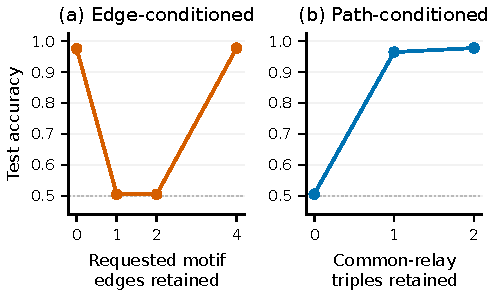
\includegraphics[width=\linewidth]{figures/edge_vs_path.pdf}
\caption{\textbf{Different structural doses can hide source-transport
differences.} (a) Requested retention of named motif edges on a real $k=4$
subgraph gives a nonmonotone response. (b) A path-conditioned edit gives a
graded response. Both zero-dose reconstructions have zero common-relay
triples, despite their different accuracies. The panels are separate
archived experiments; error bars are ten-block bootstrap 95\% intervals.}
\label{fig:edge-path}
\end{figure}

Path conditioning changes the intervention. The base graph has two
enumerated triples, one for each sink. The constrained zero-, one-, and
two-triple graphs achieve $0.5055$, $0.9641$, and $0.9772$
(Fig.~\ref{fig:edge-path}b). The full-minus-zero difference is
$0.4717$ with interval $[0.4603,0.4824]$ and corrected $q=0.0036$.
The recorded terminal-set and degree/module checks all pass. Here the
two-triple and full settings are the same retained set, so they represent
one dose, not an additional replication.

The designs also differ in deletion order and randomized partner choices.
Their task-information contrast can be inspected directly through $T$.

\subsection{Two zero-relay graphs, different source access}
\label{sec:replay}

We reconstruct the graph operators from the public MaleCNS tables and
archived extraction/intervention code. The recovered weight table matches
the original release's recorded byte count and SHA-256. The narrow base
matches 768 nodes, 44,906 dense edges, 3,072 retained edges, the five selected
motif body IDs, and the two recorded base common-relay triples. These are
post-hoc reconstruction checks; original runtime graph arrays and their
instance hashes were not retained.

Table~\ref{tab:core} places the reconstructed transfers beside the
corresponding archived outcomes. Columns of $T$ are ordered $(a,b)$ and
rows $(s_1,s_2)$.

\begin{table}[t]
\centering
\caption{\textbf{Zero common-relay count, different source access.}
Both zero-dose reconstructions preserve the base degrees/module counts
and have $|\mathcal C|=0$. Transfers are post-hoc recipe reconstructions;
accuracy and seed-bootstrap 95\% intervals are archived fit outcomes.
Original dose-instance hashes are unavailable.}
\label{tab:core}
\small
\begin{tabular}{@{}lccc@{}}
\toprule
Condition & $16T$ & Visible & Archived accuracy \\
\midrule
Base & $\left(\begin{smallmatrix}2&1\\2&1\end{smallmatrix}\right)$ & $a,b$ &
\shortstack{0.9772\\{[0.9727, 0.9820]}} \\[6pt]
Edge-zero & $\left(\begin{smallmatrix}1&0\\1&1\end{smallmatrix}\right)$ & $a,b$ &
\shortstack{0.9745\\{[0.9669, 0.9812]}} \\[6pt]
Path-zero & $\left(\begin{smallmatrix}1&0\\1&0\end{smallmatrix}\right)$ & $a$ &
\shortstack{0.5055\\{[0.4969, 0.5150]}} \\
\bottomrule
\end{tabular}
\end{table}

Both zero-dose graphs have $\mathcal C=\varnothing$ and preserve the
base degrees and module counts. The named-edge reconstruction retains
$a$ through relay 18 to both sinks and $b$ through relay 57 to $s_2$,
using compact node indices. No relay receives both sources on these
readout routes. By contrast, the path-conditioned reconstruction retains
the $a$ routes but has a zero $b$ column. Equation~\eqref{eq:criterion} assigns chance-level population accuracy
to this path-zero reconstruction. Edge-zero exposes both sources through
an invertible mixture and preserves the ideal label information.

The reconstructed source-access difference in Figure~\ref{fig:overview}
is consistent with the archived high/chance outcomes. Because both
reconstructions have the same empty common-relay family, the comparison
cannot attribute the historical gap specifically to the no-new-triple
rejection rule or isolate it from the other editing choices.

\subsection{Dose responses under two extraction rules}
\label{sec:multi}

The $k=8$ study uses broad and narrow annotation predicates and requires
at least three enumerated triples per selected source--sink configuration.
Both extractions have exactly three, giving four distinct dose levels.
Every reported dose is feasible, retains the requested terminal set, and
has zero recorded degree/module-count violations. The same ten-block task
protocol is used throughout.

\begin{figure*}[t]
\centering
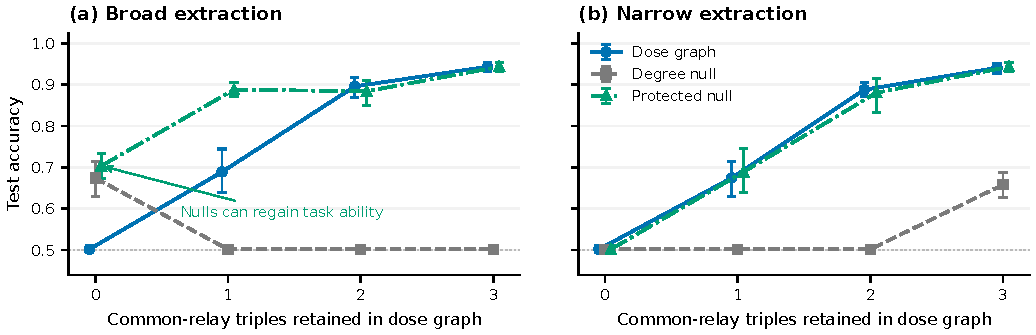
\includegraphics[width=\textwidth]{figures/multigraph.pdf}
\caption{\textbf{The dose response replicates across extraction rules, but
null behavior remains conditional.} Dose-graph accuracy increases with the
retained common-relay set in both $k=8$ extractions. Each curve includes all
four recorded doses; error bars are seed-block bootstrap 95\% intervals.
The horizontal axis specifies the dose graph's set, not the number of
triples remaining after subsequent null generation. The broad zero-dose
nulls regain task ability, and the narrow full-dose degree null is also
above chance. These exceptions prevent interpreting a degree or protection
label as functional matching.}
\label{fig:multi}
\end{figure*}

The broad extraction's dose-graph accuracies are $0.5017$, $0.6889$,
$0.8955$, and $0.9432$ for zero through three triples
(Fig.~\ref{fig:multi}a). The narrow extraction gives $0.5017$,
$0.6742$, $0.8877$, and $0.9407$
(Fig.~\ref{fig:multi}b). Full-minus-zero gaps are $0.4415$
($[0.4265,0.4542]$, corrected $q=0.0025$) and $0.4390$
($[0.4249,0.4525]$, corrected $q=0.0036$), respectively.
Direct oracle readouts reach approximately $0.999$ and linear probes
remain near chance.

The intervention changes routes while holding degrees, module counts,
and the propagation/readout architecture fixed within each extraction.
It therefore holds more statistical quantities fixed than a density change.
The reconstructed $k=8$ operators also make the remaining distinction
explicit. Broad zero dose has $64T=\left(\begin{smallmatrix}0&0\\1&0\end{smallmatrix}\right)$,
while narrow zero dose has $T=0$; both lack one or both source classes.
Every nonzero dose exposes both sources, so Eq.~\eqref{eq:criterion}
assigns all of them Bayes accuracy one in the ideal task. Their mixture
geometry and coefficients vary (full matrices are in the supplement).
Thus the graded finite-readout accuracies vary within an
information-preserving regime, rather than quantifying successive losses
of population label information.

Agreement across the two extraction rules supports robustness to this
choice of visual-neuron predicate. Both use the same animal and task
family; their 195-neuron overlap is reported in Table~\ref{tab:graphs}.
The supplement retains all seed arrays and controls.

\subsection{Protecting a path is not functional matching}
\label{sec:exceptions}

The protected null often retains task ability at the full dose: its broad
accuracy is $0.9432$, and its narrow accuracy is $0.9432$ compared with
the dose graph's $0.9407$. The latter paired graph-minus-null interval is
$[-0.0145,0.0087]$. This supports limited sensitivity to the remaining
wiring under those conditions. It does not establish equality of the
underlying functions.

More revealing are the conditions where protection is insufficient to
match behavior. In the broad zero-dose setting, the dose graph is at
$0.5017$, but the degree null reaches $0.6742$ and the protected null
$0.7032$. With no retained triples to protect, these are unrestricted
rewirings with different fixed graph-operation seeds. In the broad
one-triple setting, protection gives $0.8877$, well above the dose graph's
$0.6889$; the graph-minus-protected difference is $-0.1988$ with interval
$[-0.2483,-0.1413]$. The narrow full-dose degree null also retains
$0.6581$ accuracy.

The common-relay rejection rule
applies during dose construction, while subsequent null generation
protects a set of edges without restricting all new routes. The nulls'
task ability demonstrates that the two operations cannot be treated as
the same counterfactual. A protected null asks whether retaining those
edges allows the task after background rewiring; it does not certify
that only those edges explain the output. The two contrasts separate retaining selected routes from constraining
all surviving task information.

\subsection{What the audit changes}
\label{sec:audit-changes}

Table~\ref{tab:audit} is the protocol result. The controlled degree null removes both sources. The two zero-dose reconstructions share an empty common-relay family, but only one keeps both sources. Nonzero $k=8$ doses retain ideal label information while finite accuracy still rises. Replaying the archived seeds on the reconstructed broad zero-dose graph restores source gain $1/64$ for both nulls, matching their above-chance archived readouts.

\begin{table}[t]
\centering
\caption{\textbf{The audit changes the intervention conclusion.} Source gain
is the smaller column sum of reconstructed $T$. Ideal accuracy follows
Eq.~\eqref{eq:criterion}. Archived accuracy is the recorded finite readout.
The $k=8$ gains are computed in this revision from reconstructed graphs;
accuracies are archived.}
\label{tab:audit}
\small
\begin{tabular}{@{}lccc@{}}
\toprule
Condition & Source gain & Ideal & Archived \\
\midrule
Controlled intact & positive & 1 & 0.9971 \\
Controlled degree null & zero & 1/2 & 0.5017 \\
Named-edge zero & 0.0625 & 1 & 0.9745 \\
Path zero & 0 & 1/2 & 0.5055 \\
Broad $k=8$, zero & 0 & 1/2 & 0.5017 \\
Broad $k=8$, one & 0.015625 & 1 & 0.6889 \\
Broad $k=8$, three & 0.046875 & 1 & 0.9432 \\
Broad zero, degree null & 0.015625 & 1 & 0.6742 \\
Broad zero, protected null & 0.015625 & 1 & 0.7032 \\
\bottomrule
\end{tabular}
\end{table}

A closed-form nearest-subspace decoder confirms the ideal side of this table
without training. At zero source gain its accuracy is 0.500. At every positive
gain represented above, including $1/64$, noiseless accuracy is 1.000 on
4,096 balanced examples. Thus the finite-readout dose curve is not a curve of
ideal information loss.
\subsection{The executed readout is not a linear image of $T$}
\label{sec:images}

Nonzero columns decide the ideal subspace criterion. They do not by themselves
say what a trained nonlinear readout will do with a visual label. We therefore
attach the archived readout to the three degree- and module-matched narrow
reconstructions: a $32\!\to\!64\!\to\!1$ ReLU MLP, Adam with learning rate
0.006, 120 epochs of 32 batches of 128, and the ten recorded seeds. With
features present only at $a$ and $b$, the sink input is exactly $TX_{ab}$.
The linear control uses the same budget with the hidden layer removed.

On the subspace XOR, this replay returns MLP accuracies 0.976, 0.979, and
0.504 for the base, named-edge, and path-zero graphs
(Table~\ref{tab:executed}). The archived fits were 0.9772, 0.9745, and
0.5055. Every linear readout stays near 0.505, including on the two graphs
where the MLP exceeds 0.97. The trained model follows source visibility. A
linear image of $T$ does not solve the label.

The visual task keeps that architecture and those seeds, and replaces the Gaussian
subspaces with handwritten digits~\cite{optdigits1998}. A fixed projection maps
each 32-pixel half to 16 dimensions. Source $a$ receives an upper half, source
$b$ a lower half drawn from an independent digit, and the label is the XOR of
the two digit parities. The MLP reaches 0.746 when the columns are independent,
0.663 when they are parallel, and 0.506 when the source-$b$ column is zero.
Linear readouts remain at chance on all three graphs. Retaining both
common relays therefore does not beat an invertible pair of separate routes.
The reverse-support CIFAR-10 subset remains a negative control
(gaps $-0.0044$ and $-0.0019$).

\begin{table}[t]
\centering
\caption{\textbf{Archived MLP versus a linear readout.} Means over the ten
recorded seeds. All three graphs share degree and module counts. Linear
accuracies are 0.506, 0.505, and 0.505 on the subspace task and 0.505,
0.502, and 0.506 on the visual task, in the same row order.}
\label{tab:executed}
\small
\setlength{\tabcolsep}{3pt}
\begin{tabular}{@{}lcccc@{}}
\toprule
Graph & $|\mathcal C|$ & rank & Subspace & Visual \\
\midrule
Base & 2 & 1 & 0.976 & 0.663 \\
Named-edge zero & 0 & 2 & 0.979 & 0.746 \\
Path zero & 0 & 1 & 0.504 & 0.506 \\
\bottomrule
\end{tabular}
\end{table}

\subsection{CIFAR-10 identity follows the private column}
\label{sec:population}

A $16$-d code of an $8{\times}8$ digit is an easy class label. CIFAR-10 is not.
A two-convolution network is trained on $30{,}000$ CIFAR-10 images and then
frozen. Its $16$-d embedding is linearly classified at $0.571$ on the official
$10{,}000$-image test set. Sources $\{109,107,152,6\}$ receive independent
images through the same operator and sinks. The label is the class at one
source, so chance is $0.1$. The readout is a $32\!\to\!64\!\to\!10$ MLP, plus
a linear control, for ten seeds. Each accuracy resamples $2{,}048$ test
images. On the named-edge graph, half the energy of source $109$ lies outside
the other three columns. The base column has twice that energy and no private
component. Path zero removes it. Source $107$ keeps a shared high-gain column
on every graph.

\begin{table}[t]
\centering
\caption{\textbf{CIFAR-10 identity from four simultaneous images.} Chance is
$0.1$. The frozen embedding's own test accuracy is $0.571$. Private energy is
the residual of the labeled column. Source $109$ is deleted at these sinks
only on path zero.}
\label{tab:population}
\small
\setlength{\tabcolsep}{4pt}
\begin{tabular}{@{}llccc@{}}
\toprule
Label & Graph & Private & MLP & Linear \\
\midrule
109 & Base & 0 & 0.164 & 0.166 \\
109 & Named-edge zero & 0.00195 & 0.566 & 0.558 \\
109 & Path zero & 0 & 0.096 & 0.098 \\
107 & Base & 0 & 0.281 & 0.277 \\
107 & Named-edge zero & 0 & 0.441 & 0.434 \\
107 & Path zero & 0 & 0.440 & 0.434 \\
\bottomrule
\end{tabular}
\end{table}

Path zero reads source $107$ at $0.440$ and source $109$ at $0.096$. The
named-edge MLP reaches $0.566$, beside the embedding ceiling, and the linear
control reaches $0.558$. The base graph has more column energy and no private
direction; the MLP stays at $0.164$ and the linear control at $0.166$. The same split holds for UCI digit
identity: the named-edge MLP reaches $0.852$, path zero falls to $0.099$, and
the preserved source stays at $0.698$.
